\subsection{Source appearance transport}
\label{sec:exp_sat}
% SAT v1 paired results on the 53 clips where the appearance gate enabled it (full 526-clip pass, sheet 33). Paste only = Banksy front end without SAT.
\begin{table}[t]
\centering
\caption{\textbf{SAT on the clips where the appearance gate enables it} (53 of 526; paired, same front-end pass). $\Delta$: SAT $-$ paste only, with 95\% bootstrap CI.}
\label{tab:sat}
\small\setlength{\tabcolsep}{3pt}
\begin{tabular}{@{}lccc@{}}
\toprule
 & Paste only & + SAT & $\Delta$ [95\% CI] \\
\midrule
Readability (\%) & 98.1 & 100 & +1 clip \\
Appearance $\downarrow$ & 2.97 & 1.95 & $-1.02$ [$-1.70$, $-0.48$] \\
Flicker $\downarrow$ & 2.25 & 2.40 & $+0.15$, $p<0.001$ \\
Jitter $\downarrow$ & 8.62 & 9.42 & $+0.81$, $p=0.001$ \\
BG PSNR (dB) & 43.01 & 43.02 & n.s. \\
\bottomrule
\end{tabular}
\end{table}

% SAT: Original / paste only / + SAT (frame 24, tight crops) and the blind human study (53 SAT-enabled clips, 4 raters).
\begin{figure}[t]
\centering
\setlength{\tabcolsep}{1pt}\renewcommand{\arraystretch}{0.5}
\begin{tabular}{@{}m{1.15cm}ccc@{}}
 & \footnotesize Original & \footnotesize Paste only & \footnotesize + SAT \\[2pt]
\scriptsize \str{PHARMACY} & 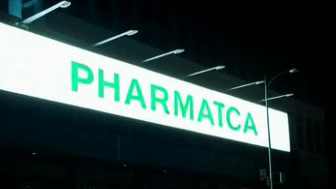
\includegraphics[width=0.265\linewidth]{figs/cells/sat_g026_en_signboard_s5_orig.jpg} & 
\includegraphics[width=0.265\linewidth]{figs/cells/sat_g026_en_signboard_s5_paste.jpg} & 
\includegraphics[width=0.265\linewidth]{figs/cells/sat_g026_en_signboard_s5_sat.jpg} \\
\scriptsize \str{CINEMA} & 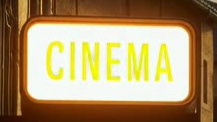
\includegraphics[width=0.265\linewidth]{figs/cells/sat_g017_en_signboard_s1_orig.jpg} & 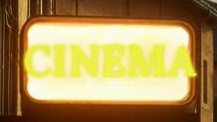
\includegraphics[width=0.265\linewidth]{figs/cells/sat_g017_en_signboard_s1_paste.jpg} & 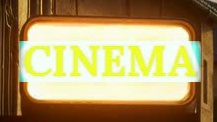
\includegraphics[width=0.265\linewidth]{figs/cells/sat_g017_en_signboard_s1_sat.jpg} \\
\scriptsize \zh{水果店} & 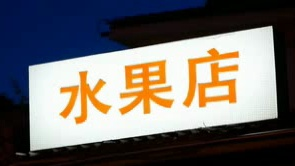
\includegraphics[width=0.265\linewidth]{figs/cells/sat_g116_zh_screen_s8_orig.jpg} & 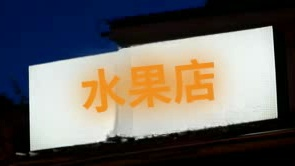
\includegraphics[width=0.265\linewidth]{figs/cells/sat_g116_zh_screen_s8_paste.jpg} & 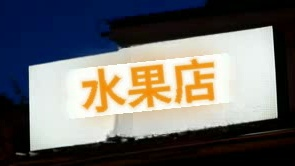
\includegraphics[width=0.265\linewidth]{figs/cells/sat_g116_zh_screen_s8_sat.jpg} \\
\scriptsize \zh{营业中}\newline\textcolor{badred}{\tiny failure} & 
\includegraphics[width=0.265\linewidth]{figs/cells/sat_g110_zh_neon_s4_orig.jpg} & 
\includegraphics[width=0.265\linewidth]{figs/cells/sat_g110_zh_neon_s4_paste.jpg} & 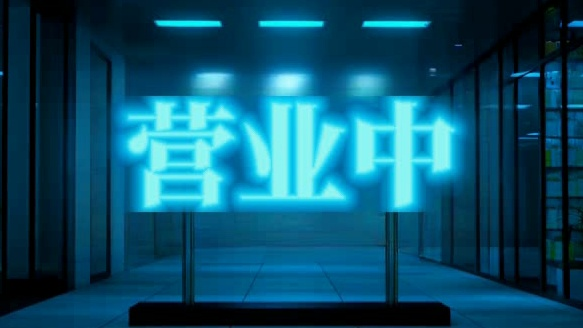
\includegraphics[width=0.265\linewidth]{figs/cells/sat_g110_zh_neon_s4_sat.jpg} \\
\end{tabular}\\[3pt]
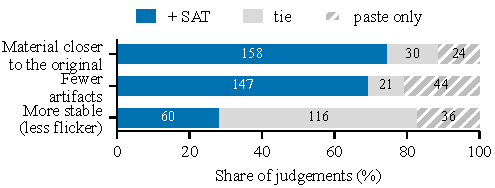
\includegraphics[width=\linewidth]{figs/plots/sat_human.pdf}
\caption{\textbf{Source appearance transport.} Top: SAT carries glow and material of the old glyphs to the new ones (rows 1--3: clips that raters judged better with SAT on both material and artifacts; row 4: a neon clip that all raters judged to have more artifacts with SAT). Bottom: blind pairwise study on all 53 SAT-enabled clips (4 raters, 212 judgements per question; \cref{sec:exp_sat}).}
\label{fig:sat}
\end{figure}


\paragraph{Where the gate enables SAT.} In the pass analysed here, the appearance gate enables SAT on 53 of the 526 clips (in the run of \cref{tab:main}, on \rSatOn): 23 of 93 neon clips, 11 of 65 screens, 9 of 86 signboards, 8 of 56 metal and 2 of 54 wooden signs, and none on glass or paper. Most rejections are clips without an accepted instance (203), followed by non-emissive text (133), no cross-validated gain (104) and gain in only one direction (33). Every enabled clip has a cross-validated error ratio below 0.75 in both directions, and the 15 rejected clips closest to the threshold lie between 0.756 and 0.795.

\paragraph{Effect.} On the enabled clips (\cref{tab:sat}), SAT reduces the appearance distance by a third ($-1.02$; better on 42 of 53 clips) for every material---screens 3.02$\to$1.33, neon 3.03$\to$2.02, wood 4.12$\to$2.21---without hurting readability or the background. It costs temporal stability: flicker rises by 0.15 and jitter by 0.81, because the transported appearance follows a per-frame distance field. On the full benchmark the readability is unchanged (90.5 vs.\ 90.3\%).

\paragraph{Human judgement.} Because the appearance distance is only a proxy, we ran a blind study on all 53 enabled clips (\cref{fig:sat}): raters saw the original between the paste-only and the SAT version in random order and answered three separate questions. Of five raters, one gave the same side on all three questions for 98\% of the clips (including the flicker question, which asks which version is worse) and was excluded by a rule (identical answers on at least 80\% of the clips) that we fixed only after seeing the data; we therefore also report the material question with all five raters. With four raters (212 judgements per question), SAT was judged closer to the original material in 158 cases against 24 (30 ties; win rate 0.87, 95\% CI [0.77, 0.94] by bootstrap over raters and clips; 48 vs.\ 3 clips by majority), and as having fewer artifacts in 147 against 44 (0.77 [0.66, 0.87]); with five raters the material win rate is 0.84 [0.74, 0.92]. Agreement is moderate (Gwet's AC1~\cite{gwet2008ac1} 0.51 for material, 0.61 for artifacts), and the left/right position had no effect after balancing (53\% left, $p=0.27$). The measured flicker increase was not perceived: 55\% of the flicker answers are ties, the remaining answers follow the material answer (a halo effect), and they correlate negatively with the measured flicker change ($\rho=-0.34$). The appearance distance agrees with the material votes only weakly ($\rho=0.28$, $p=0.049$) and not with the artifact votes, so it cannot replace human judgement.

\paragraph{Failures and their cause.} Raters judged six clips to have clearly more artifacts with SAT, four of them neon (\cref{fig:sat}, last row): a bright rectangular plate behind the new letters. A first hypothesis---that the new glyphs reach distances never observed on the old ones---was rejected (the share of unobserved distances is at most 2.3\%), and tapering the operator to identity at the edge of its support had no effect. The plates coincide instead with the canvas on which the new glyphs' distance field is computed: the canvas leaves only 0.04--0.21 letter heights of margin, so the halo, which should extend to 0.6, is cut at the canvas border. With an untruncated distance field the straight edges disappear in our diagnosis, and computing the distance field on a padded canvas reduces flicker by 0.08 and jitter by 0.37 (both better on 47 of 53 clips, $p<0.001$) with no significant change in appearance---about half of SAT's flicker cost and 40\% of its jitter cost. Because these 53 clips were used to diagnose the failure, the padded version is not part of the evaluated \method and requires validation on unseen clips.
